\chapter{Literature Review}
\label{ch:literature_review}

\section{Chapter Overview}
\label{sec:lit_chapter_overview}
Text entry and command input remain primary channels for human-computer interaction (HCI). For decades, physical keyboards and touchscreens have dominated user input. While physical keyboards provide tactile feedback that enables rapid typing, their rigid mechanical construction creates challenges \cite{ReviewVirtualKeyboard2020, Lee2022Virtual}. Physical keyboards occupy permanent desk space, cannot dynamically adapt their physical layouts for specialized workflows, and collect dirt and germs in public kiosks and hospital wards \cite{ReviewVirtualKeyboard2020}.

To overcome these physical limitations, computer vision researchers have explored virtual input devices that turn everyday planar surfaces into interactive keypads using optical sensors \cite{Zhang2001Visual, Srivastava2012RealTime, Khare2019QWERTY, Maman2023TypeNet}. Among these approaches, monocular vision keyboards that use a single standard RGB camera and a flat printed surface offer an attractive, low-cost solution because they require no specialized sensors or active electronic components.

However, implementing a dependable virtual keyboard using a single RGB camera presents several challenging computer vision and machine learning problems:
\begin{enumerate}
    \item \textbf{Surface Touch Detection Without Depth Sensors:} Standard 2D RGB cameras lack depth perception along the optical Z-axis. Detecting the precise moment when a finger makes physical contact with the paper surface, rather than hovering slightly above it, is difficult \cite{Thomas2013Camera, Posner2012Single, Lee2019Virtual, Toshpulatov2024RealTime}.
    \item \textbf{Hand Scale and Perspective Variations:} Hand landmark coordinates vary based on hand size, distance from the camera, and camera perspective \cite{Zhang2020MediaPipe, Doan2022Efficient}. Normalizing spatial landmarks without introducing temporal filtering delays is critical for detecting rapid physical impacts \cite{Kumar2026Hybrid}.
    \item \textbf{Planar Orientation and Camera Tilt:} Any tilt between the camera and the paper surface creates perspective distortion, disrupting key region mapping. Dynamic planar homography calculation ($H \in \mathbb{R}^{3 \times 3}$) is necessary to track paper position continuously \cite{Wang2016AprilTag2, Kallwies2020Determining, Pirchheim2011Homography}.
    \item \textbf{Decoupled Layout Design and Action Multiplexing:} Most prior virtual keyboards rely on fixed, hard-coded QWERTY layouts and cannot map a single printed sheet to multiple distinct action profiles \cite{ReviewVirtualKeyboard2020}.
\end{enumerate}

This chapter reviews prior research across vision-based virtual input, fiducial tracking, hand joint estimation, kinematic feature scaling, and deep learning sequence modeling. Section~\ref{sec:lit_conceptual_map} presents a conceptual taxonomy of the literature. Section~\ref{sec:lit_domain_overview} explores input hardware evolution, typing biomechanics, and ergonomic metrics. Section~\ref{sec:lit_existing_systems} analyzes existing virtual keyboard frameworks across eight sensing modalities, supported by a comparative matrix. Section~\ref{sec:lit_technological_analysis} examines key algorithms, including MediaPipe hand tracking, scale normalization, AprilTag homography, and PyTorch LSTM touch detection. Finally, Section~\ref{sec:lit_reflection} synthesizes the research gaps that motivate this thesis.

\section{Conceptual Map of the Literature}
\label{sec:lit_conceptual_map}
Figure~\ref{fig:lit_conceptual_map_diagram} illustrates the conceptual taxonomy and structural organization of the literature reviewed in this chapter.

\begin{figure}[htbp]
\centering
\resizebox{\textwidth}{!}{%
\begin{tikzpicture}[
    header/.style = {rectangle, draw=blue!80!black, fill=blue!25!white, thick, rounded corners=5pt, align=center, font=\sffamily\bfseries\small, inner sep=8pt, text width=16.5cm},
    box/.style = {rectangle, draw=blue!70!black, fill=blue!10!white, thick, rounded corners=4pt, align=center, font=\sffamily\bfseries\footnotesize, inner sep=6pt, text width=3.6cm, minimum height=1.2cm},
    subbox/.style = {rectangle, draw=gray!70, fill=gray!5!white, rounded corners=3pt, align=center, font=\sffamily\scriptsize, inner sep=5pt, text width=3.6cm},
    arrow/.style = {draw=blue!80!black, ->, >=Stealth, thick}
]

% Root Node
\node (root) [header, at={(0, 0)}] {\textbf{Monocular Vision-Based Virtual Keyboard Literature Taxonomy}};

% Level 1 Nodes
\node (l1_domain) [box, at={(-6.5, -2.0)}] {1. HCI and Input Paradigms\\(Section~\ref{sec:lit_domain_overview})};
\node (l1_systems) [box, at={(-2.15, -2.0)}] {2. Sensing Modalities\\(Section~\ref{sec:lit_existing_systems})};
\node (l1_tech) [box, at={(2.15, -2.0)}] {3. Technological Analysis\\(Section~\ref{sec:lit_technological_analysis})};
\node (l1_reflect) [box, at={(6.5, -2.0)}] {4. Research Synthesis\\(Section~\ref{sec:lit_reflection})};

% Connections to Level 1
\draw [arrow] (root.south -| l1_domain.north) -- (l1_domain.north);
\draw [arrow] (root.south -| l1_systems.north) -- (l1_systems.north);
\draw [arrow] (root.south -| l1_tech.north) -- (l1_tech.north);
\draw [arrow] (root.south -| l1_reflect.north) -- (l1_reflect.north);

% Column 1: Domain Overview
\node (l2_history) [subbox, below=0.5cm of l1_domain] {Evolution of Input Hardware\\\cite{ReviewVirtualKeyboard2020, Lee2022Virtual}};
\node (l2_drivers) [subbox, below=0.35cm of l2_history] {Paper Rationale and Ergonomics\\\cite{Zhang2001Visual, Srivastava2012RealTime, Khare2019QWERTY}};

% Column 2: Existing Systems
\node (l2_proj) [subbox, below=0.5cm of l1_systems] {Projection and IR Sensors\\\cite{Cheng2015Fingertip, Kudale2016RealTime}};
\node (l2_shadow) [subbox, below=0.35cm of l2_proj] {Shadow Analysis Methods\\\cite{Thomas2013Camera, Posner2012Single, Yue2014Blind}};
\node (l2_depth) [subbox, below=0.35cm of l2_shadow] {RGB-D / ToF Depth Sensing\\\cite{Lee2019Virtual, Toshpulatov2024RealTime}};
\node (l2_air) [subbox, below=0.35cm of l2_depth] {3D Mid-Air Typing / VR\\\cite{Boletsis2019TextInput, Enkhbat2020HandKey, Lee2022Virtual, Yoo2026WordLevel}};
\node (l2_paper) [subbox, below=0.35cm of l2_air] {Paper / Monocular RGB\\\cite{Zhang2001Visual, Srivastava2012RealTime, Khare2019QWERTY, Maman2023TypeNet}};
\node (l2_attack) [subbox, below=0.35cm of l2_paper] {Video Attack Side-Channels\\\cite{Yue2014Blind, Yang2022Towards}};

% Column 3: Technological Analysis
\node (l2_pose) [subbox, below=0.5cm of l1_tech] {MediaPipe Hand Landmarker\\\cite{Zhang2020MediaPipe, GilMartin2023Hand, Andriyanov2025Improving}};
\node (l2_scale) [subbox, below=0.35cm of l2_pose] {Hand Scale Normalization\\\cite{Doan2022Efficient, Kumar2026Hybrid}};
\node (l2_fiducial) [subbox, below=0.35cm of l2_scale] {AprilTag Homography $H$\\\cite{Wang2016AprilTag2, Kallwies2020Determining, Pirchheim2011Homography}};
\node (l2_deep) [subbox, below=0.35cm of l2_fiducial] {PyTorch LSTM Classifiers\\\cite{Hochreiter1997LSTM, Nunez2018Convolutional, Gammulle2021TMMF}};

% Column 4: Research Synthesis
\node (l2_gap) [subbox, below=0.5cm of l1_reflect] {Prior Art Limitations\\\cite{Thomas2013Camera, Lee2019Virtual, Maman2023TypeNet}};
\node (l2_solution) [subbox, below=0.35cm of l2_gap] {Proposed Architecture\\Synthesis (Section~\ref{sec:lit_reflection})};

% Vertical Column Connections
\draw [arrow] (l1_domain) -- (l2_history);
\draw [arrow] (l2_history) -- (l2_drivers);

\draw [arrow] (l1_systems) -- (l2_proj);
\draw [arrow] (l2_proj) -- (l2_shadow);
\draw [arrow] (l2_shadow) -- (l2_depth);
\draw [arrow] (l2_depth) -- (l2_air);
\draw [arrow] (l2_air) -- (l2_paper);
\draw [arrow] (l2_paper) -- (l2_attack);

\draw [arrow] (l1_tech) -- (l2_pose);
\draw [arrow] (l2_pose) -- (l2_scale);
\draw [arrow] (l2_scale) -- (l2_fiducial);
\draw [arrow] (l2_fiducial) -- (l2_deep);

\draw [arrow] (l1_reflect) -- (l2_gap);
\draw [arrow] (l2_gap) -- (l2_solution);

\end{tikzpicture}%
}
\caption{Conceptual taxonomy and structural organization of the literature review.}
\label{fig:lit_conceptual_map_diagram}
\end{figure}

The review is structured across four main themes:
\begin{itemize}
    \item \textbf{HCI and Input Paradigms (Section~\ref{sec:lit_domain_overview}):} Evolution of input hardware, biomechanics of finger-surface impact, and user performance metrics.
    \item \textbf{Sensing Modalities (Section~\ref{sec:lit_existing_systems}):} Critical evaluation of eight sensing technologies, synthesized in Table~\ref{tab:lit_comparative_matrix}.
    \item \textbf{Technological Analysis (Section~\ref{sec:lit_technological_analysis}):} Mathematical formulation and algorithmic analysis of hand tracking, scale normalization, fiducial homography, and deep learning touch detection.
    \item \textbf{Research Synthesis (Section~\ref{sec:lit_reflection}):} Identification of the six fundamental literature gaps and the formal research problem statement.
\end{itemize}

\section{Domain Overview}
\label{sec:lit_domain_overview}

\subsection{Evolution of Text Entry and Spatial HCI Hardware}
\label{subsec:lit_history_evolution}
Text entry technology has evolved across four primary generations:
\begin{enumerate}
    \item \textbf{Mechanical and Electromechanical Keyboards (1870s to 1980s):} Early mechanical typewriters and computer keyboards relied on mechanical levers and physical electrical switches \cite{ReviewVirtualKeyboard2020}. The standard QWERTY layout was engineered to separate frequently paired letters and prevent typebar jamming on mechanical typewriters, rather than optimizing typing speed or ergonomic comfort.
    \item \textbf{Membrane Keypads and Capacitive Screens (1990s to 2000s):} Membrane keyboards reduced hardware costs, while capacitive touchscreens transformed mobile computing \cite{ReviewVirtualKeyboard2020}. Touchscreens enabled dynamic software layouts, but introduced typing errors due to the complete lack of physical key edges and tactile travel.
    \item \textbf{Optical Laser Projectors and Infrared Curtains (2000s to 2010s):} Compact optical projectors displayed red laser keyboard patterns onto flat surfaces, while an infrared plane detected finger interruptions \cite{Cheng2015Fingertip, Kudale2016RealTime}. While portable, these devices proved power-hungry, suffered from optical wash-out under bright ambient light, and offered fixed, unalterable layouts.
    \item \textbf{Monocular Vision and Deep Learning Hand Tracking (2010s to Present):} Real-time neural network frameworks such as Google MediaPipe enable 21-joint skeletal hand tracking using standard RGB webcams \cite{Zhang2020MediaPipe, GilMartin2023Hand, Maman2023TypeNet}. Combining skeletal tracking with planar homography allows standard printed paper to serve as an interactive, customized virtual keyboard without extra electronics.
\end{enumerate}

\subsection{Kinematic Typing Dynamics and Biomechanical Surface Impact}
\label{subsec:lit_typing_biomechanics}
Accurate contact detection without depth sensors requires understanding the kinematics of finger impact on a rigid surface \cite{Simao2016Unsupervised, MacRitchie2015Integrating, Pilkov2024Markerless}. A physical keystroke consists of four distinct kinematic phases:
\begin{enumerate}
    \item \textbf{Approaching Phase ($t_1$ to $t_2$):} The active finger accelerates downward toward the target key, producing a sharp increase in downward vertical velocity ($V_y$).
    \item \textbf{Impact Phase ($t_2$ to $t_3$):} The fingertip collides with the rigid paper surface. Within 20 to 40 milliseconds, downward velocity drops to zero ($V_y \to 0$), producing an intense deceleration peak ($A_y = \frac{dV_y}{dt} \ll 0$).
    \item \textbf{Resting Phase ($t_3$ to $t_4$):} The finger rests momentarily on the surface while contact is registered.
    \item \textbf{Recoil Phase ($t_4$ to $t_5$):} The finger rebounds upward away from the desk, inverting vertical velocity ($V_y > 0$).
\end{enumerate}

When typing on a physical surface, the rigid tabletop provides a hard boundary that causes immediate deceleration. In contrast, in mid-air typing systems, fingers overshoot because there is no physical stopping surface \cite{Boletsis2019TextInput, Maman2023TypeNet}.

\subsection{Ergonomics and Human Input Performance Metrics}
\label{subsec:lit_fitts_law}
Text entry systems are evaluated using standard HCI metrics:
\begin{itemize}
    \item \textbf{Words Per Minute (WPM):} Typing speed is computed as $\text{WPM} = \frac{|T| - 1}{S} \times 60 \times \frac{1}{5}$, where $|T|$ is the total number of characters typed and $S$ is time in seconds.
    \item \textbf{Keystrokes Per Character (KSPC):} Measures input efficiency by comparing total keystrokes (including corrections) to generated characters. Physical keyboards average approximately 1.05 KSPC, whereas contactless mid-air keyboards often exceed 1.30 KSPC due to accidental inputs \cite{Boletsis2019TextInput}.
    \item \textbf{Fitts' Law:} Models the movement time ($MT$) required to hit a target key of width $W$ at distance $D$:
    \begin{equation}
    MT = a + b \log_2 \left( 1 + \frac{D}{W} \right) = a + b \cdot ID
    \label{eq:fitts_law}
    \end{equation}
    where $ID$ is the Index of Difficulty in bits. Customizable paper keyboards allow users to increase target key widths $W$ in the software designer, directly lowering $ID$ for users with motor impairments.
\end{itemize}

\subsection{Multi-Finger Tendon Coupling}
\label{subsec:lit_biomechanical_coupling}
In the human hand, flexor and extensor tendons are anatomically linked across adjacent fingers, particularly between the middle, ring, and pinky digits \cite{Simao2016Unsupervised, Pilkov2024Markerless}. When a user strikes a key with one finger, adjacent fingers produce involuntary sympathetic motions. Simple single-finger heuristics misinterpret these involuntary twitches as intentional key presses \cite{Thomas2013Camera, Srivastava2012RealTime}. Deep sequence models that observe temporal coordination across all joints can effectively differentiate intentional strikes from sympathetic movements.

\section{Existing Systems and Sensing Modalities}
\label{sec:lit_existing_systems}
Prior virtual input research can be grouped across eight sensing modalities.

\subsection{Projection-Based and Infrared Sensor Systems}
\label{subsec:lit_proj_systems}
Projection keyboards combine optical pattern projectors with infrared sensor grids \cite{Cheng2015Fingertip, Kudale2016RealTime}. A red laser projects keyboard outlines onto a desk, while an invisible infrared light plane projected parallel to the desk detects finger contact when breached \cite{Cheng2015Fingertip}. Kudale and Wanjale \cite{Kudale2016RealTime} implemented an infrared camera tracking reflective markers using four-point homography. While these systems avoid paper, they suffer from high power consumption, pattern wash-out under normal room lighting, and rigid, factory-fixed key layouts.

\subsection{Shadow-Based Monocular RGB Keyboards}
\label{subsec:lit_shadow_systems}
To avoid active optical hardware, earlier monocular RGB keyboards analyzed fingertip shadows \cite{Thomas2013Camera, Posner2012Single, Yue2014Blind}. Thomas \cite{Thomas2013Camera} tracked the distance between the fingertip and its cast shadow, noting that the distance reaches zero at physical contact. Posner et al. \cite{Posner2012Single} applied adaptive shadow thresholding to detect paper contacts. However, shadow analysis fails under diffuse overhead office lighting, multiple ceiling fixtures, dark desktop surfaces, or when the user's palm occludes the light source \cite{Yue2014Blind}.

\subsection{Hardware-Assisted Depth Sensors (RGB-D and ToF)}
\label{subsec:lit_depth_systems}
Specialized depth cameras, including Microsoft Kinect, Intel RealSense, and Time-of-Flight (ToF) sensors, resolve depth ambiguity by producing metric 3D point clouds \cite{Lee2019Virtual, Toshpulatov2024RealTime}. Lee and Kwon \cite{Lee2019Virtual} calibrated a planar surface to detect touch events when fingertip point clouds crossed a distance threshold. Toshpulatov et al. \cite{Toshpulatov2024RealTime} fused 3D depth data with 2D optical flow to eliminate hovering false positives. Despite their high accuracy, depth cameras are expensive, power-intensive, produce substantial close-range noise near flat surfaces, and require dedicated GPUs for real-time point cloud processing.

\subsection{3D Mid-Air Typing and AR/VR Virtual Keyboards}
\label{subsec:lit_air_systems}
Spatial computing headsets have spurred interest in mid-air keyboards \cite{Boletsis2019TextInput, Enkhbat2020HandKey, Lee2022Virtual, Yoo2026WordLevel}. Enkhbat et al. \cite{Enkhbat2020HandKey} introduced HandKey, a convolutional neural network that detects dual-hand typing within virtual 3D bounding cubes. Lee et al. \cite{Lee2022Virtual} tracked two-handed mid-air typing for head-mounted displays. However, mid-air typing causes severe arm fatigue (Gorilla Arm Syndrome) during extended sessions and lacks a physical stopping surface, causing fingers to overshoot target keys \cite{Boletsis2019TextInput, Maman2023TypeNet}.

\subsection{Paper-Anchored Monocular RGB Keyboards}
\label{subsec:lit_paper_systems}
Paper-based monocular keyboards project virtual interaction onto printed paper sheets using standard webcams \cite{Zhang2001Visual, Srivastava2012RealTime, Khare2019QWERTY, Maman2023TypeNet}. Zhang et al. \cite{Zhang2001Visual} introduced the Visual Panel, tracking paper page corners to compute homography. Srivastava and Tripathi \cite{Srivastava2012RealTime} used vertical pixel velocity thresholds to detect key presses. Khare \cite{Khare2019QWERTY} tracked a printed QWERTY sheet using skin-color segmentation. Recently, TypeNet \cite{Maman2023TypeNet} demonstrated touch typing on uncalibrated surfaces using deep keypoint tracking and language model decoding. However, these systems rely on fixed QWERTY layouts, require users to hold their fingers over keys for artificial dwell times, and lose tracking when the paper shifts.

\subsection{Specialized and Assistive Modalities}
\label{subsec:lit_specialized_assistive}
Alternative sensing approaches include Visible Light Communication (VLC) photodiode arrays \cite{Webber2021Finger}, fingernail blood volume deformation imaging \cite{Sun2009Estimation}, multi-camera optical motion capture \cite{MacRitchie2015Integrating, Pilkov2024Markerless}, and eye-gaze tracking \cite{Chen2024Gaze}. While assistive eye-gaze systems help motor-impaired individuals, they suffer from the Midas Touch problem, where pauses to read text trigger unwanted inputs \cite{Chen2024Gaze}.

\subsection{Fiducial Tracking in Planar Robotics}
\label{subsec:lit_robotics_systems}
Planar tracking using fiducial markers is widely used in robotic servoing \cite{Ivacko2024Edge, Herdiansyah2024Implementation, Schenck2024Utilizing, GarridoJurado2026ArUco}. Ivacko et al. \cite{Ivacko2024Edge} used ArUco markers to map robot arm coordinate frames. Garrido-Jurado et al. \cite{GarridoJurado2026ArUco} introduced ArUco Nano, achieving high frame rates using contour scanning. These robotics studies demonstrate that visual fiducials provide robust sub-pixel planar localization under perspective tilt, making them well-suited for paper keyboard tracking.

\subsection{Comparative Literature Analysis Matrix}
\label{subsec:lit_comparative_matrix}
Table~\ref{tab:lit_comparative_matrix} summarizes representative prior works across sensing modality, hardware requirements, tracking method, scale normalization, temporal filtering, touch classification, and layout flexibility.

\begin{table}[htbp]
\centering
\caption{Comparative analysis of existing virtual keyboard frameworks and sensing methodologies.}
\label{tab:lit_comparative_matrix}
\resizebox{\textwidth}{!}{%
\begin{tabular}{l l l l l l l l l}
\toprule
\textbf{Study and Year} & \textbf{Sensing Modality} & \textbf{Hardware Req.} & \textbf{Surface Tracking} & \textbf{Scale Normalization} & \textbf{Temporal Filter} & \textbf{Touch Classifier} & \textbf{Latency / FPS} & \textbf{Layout Customization} \\
\midrule
Zhang et al. (2001) \cite{Zhang2001Visual} & Monocular RGB & Standard Webcam & Quad Paper Bounds & None (Pixel Coords) & Moving Avg. & Spatial Proximity & High ($\sim 15$ FPS) & Rigid Paper Quad \\
Sun et al. (2009) \cite{Sun2009Estimation} & Monocular RGB & High-Res Camera & None (Fixed Finger) & None & None & LDA Nail Coloration & Offline ($< 5$ FPS) & None \\
Pirchheim and Reitmayr (2011) \cite{Pirchheim2011Homography} & Monocular RGB & Mobile Camera & Keyframe Homography & Feature Scale & Particle Filter & Spatial Tracking & Real-Time ($30$ FPS) & None (SLAM Map) \\
Srivastava and Tripathi (2012) \cite{Srivastava2012RealTime} & Monocular RGB & Standard Webcam & Manual Quad Contour & None (Raw Pixels) & Static Smoothing & Speed Deceleration & Real-Time ($25$ FPS) & Manual Paper Drawing \\
Posner et al. (2012) \cite{Posner2012Single} & Monocular RGB & Standard Webcam & Fixed Desk Layout & None & Dynamic Threshold & Fingertip-Shadow Dist. & Real-Time ($30$ FPS) & Fixed Paper Template \\
Thomas (2013) \cite{Thomas2013Camera} & Monocular RGB & Standard Webcam & Fixed Area & None & None & Shadow Gradient Vector & Real-Time ($30$ FPS) & Fixed Layout \\
Yue et al. (2014) \cite{Yue2014Blind} & Monocular RGB & Smartphone RGB & Screen Border H & None & Optical Flow & Shadow + k-Means & Offline Analysis & Fixed Smartphone Screen \\
Cheng et al. (2015) \cite{Cheng2015Fingertip} & Proj. + Camera & Projector + Camera & Photometric Calib. & None & Background Sub. & 3D Shadow Distance & Real-Time ($20$ FPS) & Fixed Projected GUI \\
MacRitchie and McPherson (2015) \cite{MacRitchie2015Integrating} & Optical MoCap & MoCap + Touch & Surface Calibration & 3D Skeleton mm & Moving Average & Velocity Inversion & Real-Time ($100$ FPS) & Fixed Piano Keys \\
Kudale and Wanjale (2016) \cite{Kudale2016RealTime} & IR Webcam & IR Filtered Camera & 4-Point Homography & None & Thresholding & IR Pen Tap Contact & Real-Time ($30$ FPS) & Projected Display \\
Simao et al. (2017) \cite{Simao2016Unsupervised} & Motion Capture & Leap Motion Sensor & None & Bone Lengths & Sliding Window & Velocity Inversion & Real-Time ($60$ FPS) & None \\
Ji et al. (2018) \cite{Ji2018Local} & Monocular RGB & Standard Webcam & Skin Color Mask & None & Moving Avg. & k-Means Clustering & Real-Time ($25$ FPS) & Dynamic Key Clusters \\
Nunez et al. (2018) \cite{Nunez2018Convolutional} & 3D Skeleton & Depth Sensor & None & Normalized Skeleton & Sequence Window & CNN + LSTM Network & Real-Time ($30$ FPS) & None \\
Lai and Yanushkevich (2018) \cite{Lai2018CNN} & Multimodal RGB-D & Depth Sensor & None & Skeleton Joint Map & Temporal Buffer & CNN + RNN Fusion & Real-Time ($30$ FPS) & Gesture Set \\
Khare (2019) \cite{Khare2019QWERTY} & Monocular RGB & Standard Webcam & Static Bounds & None & Color Threshold & Pause Over Bounds & Real-Time ($20$ FPS) & Fixed QWERTY Paper \\
Lee and Kwon (2019) \cite{Lee2019Virtual} & RGB-D Depth & ToF Depth Camera & Depth Plane Calib. & 3D Metric mm & Weight Filtering & Z-Depth Threshold & Real-Time ($30$ FPS) & Fixed Virtual Touch \\
Boletsis and Kongsvik (2019) \cite{Boletsis2019TextInput} & VR Controller & VR Headset & Virtual 3D Grid & VR World Scale & None & Striking Velocity & Real-Time ($90$ FPS) & Fixed VR Layout \\
Enkhbat et al. (2020) \cite{Enkhbat2020HandKey} & Monocular RGB & Standard Webcam & Air Typing Zone & Hand Size Scaling & None & CNN Spatial Classifier & Real-Time ($30$ FPS) & Fixed Air QWERTY \\
Cui et al. (2020) \cite{Cui2020Deep} & Vision Review & Various Sensors & Various & Various & Various & Deep Learning Survey & N/A & N/A \\
Zhang et al. (2020) \cite{Zhang2020MediaPipe} & Monocular RGB & Commodity Camera & Palm Detector & Normalized 21 Keypoints & Single-frame Regress & Skeletal Keypoint Reg. & High Speed ($> 60$ FPS) & General Hand Tracking \\
Ikram and Liu (2020) \cite{Ikram2020Skeleton} & 3D Skeleton & Leap Motion Sensor & None & Hand Scale & Sliding Window & 1D CNN + LSTM & Real-Time ($50$ FPS) & Mid-air Gestures \\
Wang et al. (2020) \cite{Wang2020Relative} & Monocular RGB & Stereo Pair & Superpixel Homography & Superpixel Scale & Bundle Adjust & Multi-Model RANSAC & Real-Time ($25$ FPS) & Planar Maps \\
Li et al. (2021) \cite{Li2021CNN} & Monocular RGB & Embedded Camera & Grid Mask & None & CNN Feature Map & Lightweight CNN & Edge Real-Time ($30$ FPS) & Fixed Key Grid \\
Webber et al. (2021) \cite{Webber2021Finger} & Visible Light & VLC Photodiodes & Optical Intensity Mask & None & Intensity Features & SVM / Random Forest & Real-Time ($30$ FPS) & Light Grid Keys \\
Gammulle et al. (2021) \cite{Gammulle2021TMMF} & Multimodal RGB & Single Camera & None & Sequence Normalization & Multi-Modal Fusion & Single-Stage TMMF Net & Real-Time ($30$ FPS) & Continuous Gestures \\
Zhang et al. (2022) \cite{Zhang2022DynaKey} & Head-Mounted RGB & Smart Glasses & Gyro + Homography & None & Motion Compensation & Downward Trajectory & Real-Time ($30$ FPS) & Drawn Keyboard Bounds \\
Lee et al. (2022) \cite{Lee2022Virtual} & RGB-D / HMD & AR/VR Headset & HMD Frame & 3D Joint Scaling & Temporal Buffer & 7-Class Deep Network & Real-Time ($60$ FPS) & Ambidextrous Layouts \\
Doan (2022) \cite{Doan2022Efficient} & Monocular RGB & Commodity RGB & None & Scale Normalized & Coordinate Smooth & Multi-layer LSTM & Real-Time ($30$ FPS) & Body Activity \\
Yang et al. (2022) \cite{Yang2022Towards} & Smartphone RGB & Commodity Phone & Uncalibrated Video & Self-Supervised Scale & Motion Trajectory & Deep Inference Model & Offline Analysis & Uncalibrated Keyboards \\
Maman and Bermano (2023) \cite{Maman2023TypeNet} & Monocular RGB & Front Camera & Uncalibrated Plane & Hand Skeleton Scale & Self-Refinement & Deep Net + LM Decoding & Real-Time ($30$ FPS) & Fixed QWERTY Flat \\
Gil-Martin et al. (2023) \cite{GilMartin2023Hand} & Monocular RGB & Commodity Camera & None & MediaPipe Scale & Sequence Buffer & Deep Recurrent Net & Real-Time ($60$ FPS) & General Gestures \\
Sanchez-Brizuela et al. (2023) \cite{SanchezBrizuela2023Lightweight} & Monocular RGB & Commodity Camera & None & Landmark Distance & Morphological Mask & Landmark Rule Classifier & Ultra High ($90$ FPS) & Skin Segmentation \\
Ivacko et al. (2024) \cite{Ivacko2024Edge} & Monocular RGB & Wrist Camera & ArUco Calibration & Metric Scaling & Low-Pass Alpha & Rule-Based Kinematics & Edge Real-Time ($30$ FPS) & Robot Control Pad \\
Herdiansyah et al. (2024) \cite{Herdiansyah2024Implementation} & Monocular RGB & Single RGB Camera & ArUco PnP & Metric Tag Size & Zhang Calibration & Geometric Pose Engine & Real-Time ($30$ FPS) & Navigation Targets \\
Pilkov (2024) \cite{Pilkov2024Markerless} & Multi-Camera RGB & 3 RGB Cameras & None & 3D Skeleton mm & Temporal Alignment & Deep Keypoint Trajectory & Real-Time ($30$ FPS) & Piano Keyboard \\
Toshpulatov et al. (2024) \cite{Toshpulatov2024RealTime} & Multimodal RGB-D & Depth + RGB & Surface Calib. & 3D Spatial mm & Fusion Filter & Temporal Depth-Motion Net & Real-Time ($30$ FPS) & VR/AR GUI Objects \\
Chen (2024) \cite{Chen2024Gaze} & Monocular RGB & Commodity Webcam & Screen Grid & Pupil Vector Scale & Dwell Time Filter & Eye-Gaze Deep Model & Real-Time ($30$ FPS) & Gaze Keypad \\
Schenck et al. (2024) \cite{Schenck2024Utilizing} & Monocular RGB & Single RGB Camera & ArUco Inpainting & Metric Scale & Inpainting Mask & Deep Keypoint Detector & Real-Time ($30$ FPS) & Robotic Links \\
Andriyanov et al. (2025) \cite{Andriyanov2025Improving} & Monocular RGB & Commodity RGB & Bounding Box & Normalized Bounds & Temporal Window & MediaPipe + YOLO-Pose & Real-Time ($45$ FPS) & Gesture Set \\
Yoo and Lee (2026) \cite{Yoo2026WordLevel} & Monocular RGB & Single RGB Camera & None & Trajectory Scaling & Displacement Accum. & Word Motion Network & Real-Time ($30$ FPS) & Contactless QWERTY \\
Kumar (2026) \cite{Kumar2026Hybrid} & Monocular RGB & Commodity Camera & Canvas Plane & Landmark Ratio & Adaptive Low-Pass & Motion Threshold & Real-Time ($60$ FPS) & Air Canvas Drawing \\
Garrido-Jurado et al. (2026) \cite{GarridoJurado2026ArUco} & Monocular RGB & Commodity Camera & ArUco Nano Tags & Metric Tag Scale & Sub-pixel Sampling & Visited-Aware Contours & Edge High ($> 100$ FPS) & Robotics Targets \\
\bottomrule
\end{tabular}%
}
\end{table}

\section{Technological Analysis}
\label{sec:lit_technological_analysis}
This section analyzes the four foundational technical modules: skeletal hand tracking, scale normalization, planar homography, and deep learning touch classification.

\subsection{Hand Pose Estimation and Skeletal Joint Tracking}
\label{subsec:lit_hand_pose}
Markerless 2D and 3D hand tracking is essential for natural input \cite{Cui2020Deep, Zhang2020MediaPipe}. While early systems used color segmentation in HSV or YCbCr spaces \cite{Ji2018Local, Khare2019QWERTY}, color thresholding breaks down under variable lighting and diverse skin tones.

Google MediaPipe Hands \cite{Zhang2020MediaPipe} addresses these issues using a two-stage machine learning pipeline optimized for standard CPUs:
\begin{enumerate}
    \item \textbf{Single-Shot Palm Detector:} Detects a 2D oriented bounding box around the palm across the full frame using focal loss $\mathcal{L}_{\text{focal}} = -\alpha_t (1 - p_t)^\gamma \log(p_t)$. By focusing on the rigid palm rather than articulating fingers, it minimizes detection failures.
    \item \textbf{Hand Landmark Model:} Operates on the cropped palm region to predict 3D coordinates $(x_i, y_i, z_i)$ for 21 skeletal joints (Figure~\ref{fig:mediapipe_hand_topology}).
\end{enumerate}

\begin{figure}[htbp]
\centering
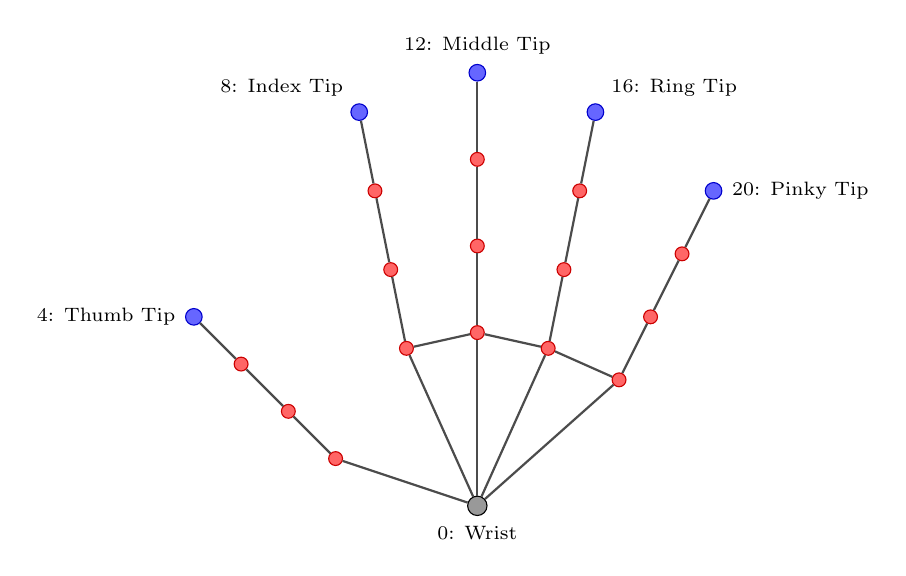
\begin{tikzpicture}[
    joint/.style = {circle, draw=red!80!black, fill=red!60!white, inner sep=0pt, minimum size=5pt},
    tip/.style = {circle, draw=blue!80!black, fill=blue!60!white, inner sep=0pt, minimum size=6pt},
    wrist/.style = {circle, draw=black, fill=gray!80, inner sep=0pt, minimum size=7pt},
    bone/.style = {draw=black!70, thick}
]

% Wrist
\node (J0) [wrist, label=below:{\scriptsize 0: Wrist}] at (0, 0) {};

% Thumb
\node (J1) [joint] at (-1.8, 0.6) {};
\node (J2) [joint] at (-2.4, 1.2) {};
\node (J3) [joint] at (-3.0, 1.8) {};
\node (J4) [tip, label=left:{\scriptsize 4: Thumb Tip}] at (-3.6, 2.4) {};

% Index Finger
\node (J5) [joint] at (-0.9, 2.0) {};
\node (J6) [joint] at (-1.1, 3.0) {};
\node (J7) [joint] at (-1.3, 4.0) {};
\node (J8) [tip, label=above left:{\scriptsize 8: Index Tip}] at (-1.5, 5.0) {};

% Middle Finger
\node (J9) [joint] at (0.0, 2.2) {};
\node (J10) [joint] at (0.0, 3.3) {};
\node (J11) [joint] at (0.0, 4.4) {};
\node (J12) [tip, label=above:{\scriptsize 12: Middle Tip}] at (0.0, 5.5) {};

% Ring Finger
\node (J13) [joint] at (0.9, 2.0) {};
\node (J14) [joint] at (1.1, 3.0) {};
\node (J15) [joint] at (1.3, 4.0) {};
\node (J16) [tip, label=above right:{\scriptsize 16: Ring Tip}] at (1.5, 5.0) {};

% Pinky Finger
\node (J17) [joint] at (1.8, 1.6) {};
\node (J18) [joint] at (2.2, 2.4) {};
\node (J19) [joint] at (2.6, 3.2) {};
\node (J20) [tip, label=right:{\scriptsize 20: Pinky Tip}] at (3.0, 4.0) {};

% Bones Connections
\draw [bone] (J0) -- (J1) -- (J2) -- (J3) -- (J4);
\draw [bone] (J0) -- (J5) -- (J6) -- (J7) -- (J8);
\draw [bone] (J0) -- (J9) -- (J10) -- (J11) -- (J12);
\draw [bone] (J0) -- (J13) -- (J14) -- (J15) -- (J16);
\draw [bone] (J0) -- (J17) -- (J18) -- (J19) -- (J20);
\draw [bone] (J5) -- (J9) -- (J13) -- (J17);

\end{tikzpicture}
\caption{MediaPipe 21 hand landmark anatomical topology.}
\label{fig:mediapipe_hand_topology}
\end{figure}

MediaPipe provides five fingertip coordinates (Landmarks 4, 8, 12, 16, 20) and knuckle base joints (MCP, PIP, DIP) at execution speeds exceeding 60 FPS on standard CPUs \cite{GilMartin2023Hand, SanchezBrizuela2023Lightweight}.

\subsection{Kinematic Scale Normalization and Raw Feature Propagation}
\label{subsec:lit_scale_norm}
Raw landmark pixel coordinates vary with hand distance from the camera and physical hand size \cite{Doan2022Efficient, Kumar2026Hybrid}. Under the standard pinhole camera projection model:
\begin{equation}
x_{\text{pixel}} = f \frac{X}{Z}, \quad y_{\text{pixel}} = f \frac{Y}{Z}
\label{eq:pinhole_projection}
\end{equation}

When the distance between hand and camera changes by factor $k$ ($Z' = k Z$), image plane coordinates scale inversely:
\begin{equation}
x'_{\text{pixel}} = \frac{x_{\text{pixel}}}{k}, \quad y'_{\text{pixel}} = \frac{y_{\text{pixel}}}{k}, \quad L'_{\text{hand}} = \frac{L_{\text{hand}}}{k}
\label{eq:pixel_scaling}
\end{equation}
where $L_{\text{hand}}$ is the reference hand length defined as the Euclidean distance between the wrist $\mathbf{P}_0 = (x_0, y_0)$ and the middle MCP knuckle $\mathbf{P}_9 = (x_9, y_9)$:
\begin{equation}
L_{\text{hand}} = \sqrt{(x_9 - x_0)^2 + (y_9 - y_0)^2}
\label{eq:hand_length_scale_def}
\end{equation}

Normalizing landmark coordinates relative to the wrist reference $\mathbf{P}_0$ and dividing by $L_{\text{hand}}$ eliminates scale dependency:
\begin{equation}
\mathbf{P}_i^{\text{norm}\prime} = \frac{\mathbf{P}_i' - \mathbf{P}_0'}{L'_{\text{hand}}} = \frac{\frac{\mathbf{P}_i - \mathbf{P}_0}{k}}{\frac{L_{\text{hand}}}{k}} = \frac{\mathbf{P}_i - \mathbf{P}_0}{L_{\text{hand}}} = \mathbf{P}_i^{\text{norm}}
\label{eq:scale_invariance_proof}
\end{equation}

First-order numerical velocities are computed across consecutive frames:
\begin{equation}
\mathbf{V}_i(t) = \frac{\mathbf{P}_i^{\text{norm}}(t) - \mathbf{P}_i^{\text{norm}}(t - \Delta t)}{\Delta t}
\label{eq:joint_velocity_def}
\end{equation}

Unlike mid-air gesture systems that apply low-pass or moving-average filters to smooth jitter \cite{Kumar2026Hybrid}, surface touch detection requires direct feature propagation without temporal filtering. Smoothing filters flatten the abrupt deceleration peak ($A_y \ll 0$) that occurs within 40 ms of surface contact, causing missed touches and adding 30 to 90 ms of latency delay.

\subsection{Planar Homography and Fiducial Tracking}
\label{subsec:lit_homography}
Mapping camera pixels $(x_{\text{pixel}}, y_{\text{pixel}})$ to the printed paper layout plane $(x_{\text{XML}}, y_{\text{XML}})$ requires correcting for perspective distortion \cite{LonguetHiggins1985Machine, Pirchheim2011Homography, Wang2020Relative}. Projective geometry maps points between two coplanar surfaces through a $3 \times 3$ planar homography matrix $H$:
\begin{equation}
\begin{bmatrix}
x_{\text{XML}} w \\
y_{\text{XML}} w \\
w
\end{bmatrix}
=
H \mathbf{P}_{\text{pixel}}
=
\begin{bmatrix}
h_{11} & h_{12} & h_{13} \\
h_{21} & h_{22} & h_{23} \\
h_{31} & h_{32} & h_{33}
\end{bmatrix}
\begin{bmatrix}
x_{\text{pixel}} \\
y_{\text{pixel}} \\
1
\end{bmatrix}
\label{eq:homography_equation_def}
\end{equation}

Cartesian coordinates on the layout sheet are recovered by normalizing by scale factor $w$:
\begin{equation}
x_{\text{XML}} = \frac{h_{11} x_{\text{pixel}} + h_{12} y_{\text{pixel}} + h_{13}}{h_{31} x_{\text{pixel}} + h_{32} y_{\text{pixel}} + h_{33}}, \quad
y_{\text{XML}} = \frac{h_{21} x_{\text{pixel}} + h_{22} y_{\text{pixel}} + h_{23}}{h_{31} x_{\text{pixel}} + h_{32} y_{\text{pixel}} + h_{33}}
\label{eq:homography_cartesian_def}
\end{equation}

Using four point correspondences between known marker corners and camera image coordinates, the Direct Linear Transform (DLT) produces a linear system $\mathbf{A}_{8 \times 9} \mathbf{h} = \mathbf{0}$, which is solved via Singular Value Decomposition (SVD) \cite{Wang2016AprilTag2, Kallwies2020Determining}.

Comparative studies by Kalaitzakis et al. \cite{Kalaitzakis2021Fiducial} demonstrate that AprilTag achieves a lower corner localization error (0.017 pixels) than ArUco and ARTag under camera tilts up to $75^\circ$. Moreover, AprilTag executes in under 1.0 ms on standard CPUs, making it ideal for real-time tracking without GPU hardware.

\subsection{Deep Sequential Touch Detection Models}
\label{subsec:lit_deep_touch}
Thresholding velocity alone ($V_y > \theta$) fails to reliably identify touch events due to hand hovering and tendon coupling \cite{Simao2016Unsupervised, Toshpulatov2024RealTime}. Long Short-Term Memory (LSTM) recurrent networks \cite{Hochreiter1997LSTM} maintain internal memory across temporal sequences, making them well-suited for kinematic impact classification:
\begin{align}
\mathbf{f}_t &= \sigma(\mathbf{W}_f [\mathbf{h}_{t-1}, \mathbf{x}_t] + \mathbf{b}_f) \label{eq:lstm_forget_def} \\
\mathbf{i}_t &= \sigma(\mathbf{W}_i [\mathbf{h}_{t-1}, \mathbf{x}_t] + \mathbf{b}_i) \label{eq:lstm_input_def} \\
\tilde{\mathbf{C}}_t &= \tanh(\mathbf{W}_c [\mathbf{h}_{t-1}, \mathbf{x}_t] + \mathbf{b}_c) \label{eq:lstm_candidate_def} \\
\mathbf{C}_t &= \mathbf{f}_t \odot \mathbf{C}_{t-1} + \mathbf{i}_t \odot \tilde{\mathbf{C}}_t \label{eq:lstm_cell_def} \\
\mathbf{o}_t &= \sigma(\mathbf{W}_o [\mathbf{h}_{t-1}, \mathbf{x}_t] + \mathbf{b}_o) \label{eq:lstm_output_def} \\
\mathbf{h}_t &= \mathbf{o}_t \odot \tanh(\mathbf{C}_t) \label{eq:lstm_hidden_def}
\end{align}

Temporal sequence models evaluate hand kinematics across sliding windows of 5 frames with 2-frame overlap (a stride of 3 frames). At a 12 FPS sampling rate, a 5-frame window covers 416.6 ms, capturing downward descent, surface contact, and rebound while keeping CPU inference latency under 4 ms per window.

\subsection{System Architecture Sensing Trade-Offs}
\label{subsec:lit_sensing_tradeoffs}
Table~\ref{tab:lit_sensing_tradeoffs} compares the architectural trade-offs between the proposed monocular RGB approach and other sensing modalities.

\begin{table}[htbp]
\centering
\caption{System architecture design trade-offs across sensing modalities.}
\label{tab:lit_sensing_tradeoffs}
\resizebox{\textwidth}{!}{%
\begin{tabular}{l l l l l}
\toprule
\textbf{Architectural Dimension} & \textbf{Monocular RGB + AprilTag (Proposed)} & \textbf{RGB-D / ToF Depth Sensing} & \textbf{Laser Projection + IR} & \textbf{3D Mid-Air Typing (VR)} \\
\midrule
\textbf{Hardware Sensor Cost} & Low (Commodity Webcam) & High (\$150 to \$400 Depth Camera) & Medium (\$80 to \$150 Projector) & High (\$400 to \$3500 Headset) \\
\textbf{Ambient Light Sensitivity} & Moderate (Robust to indoor lux) & High (Sunlight IR interference) & Extreme (Sunlight washes pattern) & Low (Built-in HMD sensors) \\
\textbf{Surface Alignment} & Dynamic (AprilTag Homography) & Fixed Depth Plane Calibration & Fixed Desktop Projection & None (Mid-air tracking) \\
\textbf{Tactile Feedback} & Passive Surface Tactile Stop & Passive Surface Tactile Stop & Passive Surface Tactile Stop & Complete Absence (Fatigue) \\
\textbf{Layout Customization} & High (Printable XML Layouts) & Moderate (Fixed Spatial GUI) & Low (Hardcoded Laser Pattern) & High (Software VR Grids) \\
\textbf{Edge Compute Latency} & Low ($> 60$ FPS on CPU) & Medium (Point Cloud Compute) & Low (Hardware IR Processing) & High (Heavy HMD Pipeline) \\
\bottomrule
\end{tabular}%
}
\end{table}

As shown in Table~\ref{tab:lit_sensing_tradeoffs}, combining a standard monocular webcam with AprilTag tracking balances hardware accessibility, planar stability, passive tactile contact, and flexible layout customization.

\section{Reflection and Synthesis of Research Gaps}
\label{sec:lit_reflection}

\subsection{Synthesis of Prior Literature Limitations}
\label{subsec:lit_synthesis_limitations}
Our review reveals six primary limitations in existing virtual keyboard systems:
\begin{enumerate}
    \item \textbf{Single-Finger Tracking Restrictions:} Prior monocular systems track only one active finger at a time (typically the index finger or the fastest moving digit) \cite{Thomas2013Camera, Ji2018Local, Srivastava2012RealTime}. Shadow-based techniques fail when multiple fingers move together because shadows merge and occlude one another \cite{Posner2012Single}.
    \item \textbf{Artificial Dwell-Time Delays:} Lacking reliable depth perception, earlier 2D systems required users to freeze their finger over a key for 500 to 1000 ms to confirm a press \cite{Khare2019QWERTY, Chen2024Gaze}. This artificial delay disrupts natural typing flow.
    \item \textbf{High Computational Overhead and GPU Dependencies:} Deep learning vision frameworks often require dedicated GPUs to run in real time, dropping below 15 FPS when executed on standard commodity CPUs \cite{Enkhbat2020HandKey, Ji2018Local}.
    \item \textbf{Brittleness Under Lighting and Shadow Variations:} Shadow tracking and skin-color thresholding break down under diffuse indoor lighting, multiple light sources, soft ambient hand shadows, and diverse skin tones \cite{Thomas2013Camera, Yue2014Blind}.
    \item \textbf{Reliance on Specialized Hardware:} Resolving depth ambiguity in prior systems often required expensive Time-of-Flight sensors, stereo cameras, infrared projectors, or sensor gloves \cite{Lee2019Virtual, Kudale2016RealTime, Toshpulatov2024RealTime, Pilkov2024Markerless}.
    \item \textbf{Rigid Layouts and Lack of Action Multiplexing:} Existing vision keyboards hard-code fixed QWERTY layouts into their applications \cite{Maman2023TypeNet, Enkhbat2020HandKey}. They cannot generate custom printed sheets with fiducial anchors or bind multiple distinct software actions to the same physical layout sheet.
\end{enumerate}

\subsection{Formal Research Gap Justification}
\label{subsec:lit_gap_justification}
These limitations establish the core research gap addressed by this thesis:

\begin{quote}
\emph{The absence of an integrated, real-time virtual keyboard framework operating strictly on a single standard monocular RGB camera and commodity CPU, using standard printed paper without active electronics, that detects independent multi-finger touch impacts without artificial dwell delays, dynamically compensates for paper displacement via planar homography, and enables a single printed layout sheet to be dynamically multiplexed across diverse software action profiles at regular camera resolutions.}
\end{quote}

By combining custom layout design, AprilTag homography, unitless hand-length scale normalization ($L_{\text{hand}}$), direct feature propagation, and a lightweight PyTorch LSTM touch classifier, this thesis addresses these limitations directly.

\section{Chapter Summary}
\label{sec:lit_chapter_summary}
This chapter reviewed prior literature across virtual input devices, hand pose estimation, fiducial planar tracking, and deep learning touch classification. Section~\ref{sec:lit_conceptual_map} provided a conceptual map of the domain. Section~\ref{sec:lit_domain_overview} outlined the history of input hardware, impact biomechanics, and ergonomic metrics. Section~\ref{sec:lit_existing_systems} evaluated eight sensing modalities and summarized them in a comparative matrix. Section~\ref{sec:lit_technological_analysis} analyzed the mathematical foundations of MediaPipe pose estimation, scale normalization, AprilTag homography, and LSTM sequence classification. Finally, Section~\ref{sec:lit_reflection} synthesized the six research gaps motivating this research. These foundations inform the methodology and system architecture presented in Chapter~\ref{ch:methodology}.
